\documentclass[frontgrid]{flacards}
% For sets e.g. \mathbb{Z}
\usepackage{amsfonts}
% For the 'split' envirnoment and symbols
\usepackage{amsmath, amssymb}
% For grey outs in the 'flashcard' environment
\usepackage{color}
% For parse trees
\usepackage{proof}
% For venn diagrams
\usepackage{tikz}
% Multi line tables
\usepackage{tabularx}
% For tikz backgrounds (i.e. filling in S!)
\usetikzlibrary{backgrounds,positioning}

\definecolor{light-gray}{gray}{0.75}

\newcommand{\frontcard}[1]{\textcolor{light-gray}{\colorbox{light-gray}{$#1$}}}
\newcommand{\backcard}[1]{#1} 

\newcommand{\flashcard}[1]{% create new command for cards with blanks
    \card{% call the original \card command with twice the same argument (#1)
        \let\blank\frontcard% but let \blank behave like \frontcard the first time
        #1
    }{%
        \let\blank\backcard% and like \backcard the second time
        #1
    }%
}

% Venn diagram circles
\def\firstcircle{(0:0.8cm) circle (1.2cm)}
\def\secondcircle{(180:0.8cm) circle (1.2cm)}
\def\thirdcircle{(0:0.4cm) circle (0.4cm)}

% Gives us a dot to use in parse trees. The phantom '|' symbols aren't shown but
% give us vertical (and a little bit of horizontal) space so the parse tree has
% the correct spacing.
\newcommand{\parsetreedot}{\phantom{|}\cdot\phantom{|}}

\begin{document}

\pagesetup{2}{6} 

% The basic sets

\card{
	The set $\mathbb{N}$ contains?
}{
	The set of natural numbers (all non-negative integers).
}

\card{
	The set $\mathbb{R}$ contains?
}{
	The set of real numbers (all finite and infinite decimal numbers).
}

\card{
	The set $\mathbb{Z}$ contains?
}{
	The set of integers.
}

\card{
	The set $\mathbb{Q}$ contains?
}{
	The set of rational numbers.\\
	Contains all $m/n$ for $m, n \in \mathbb{Z}$
}

\card{
	What is this?\\$\emptyset$
}{
	The null set.
}

\card{
	What is this?\\$\mathbb{S}$
}{
	The universal set, containing all possible elements.
}

% Set operations

\card{
	What does $X \subseteq Y$ mean?
}{
	$X$ is a subset of $Y$\\
	$Y$ is a superset of $X$\\
	$X$ is included in $Y$\\
	$Y$ includes $X$\\
	\vspace{3mm}
    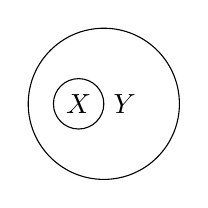
\begin{tikzpicture}[scale=0.8]
      \draw \firstcircle node[text=black,right] {$Y$};
      \draw \thirdcircle node [text=black] {$X$};
    \end{tikzpicture}
}

\card{
	What does $'$ mean after a set (or $^{c}$)?
}{
	The complement of the set. E.g. $X'$:\\
	\vspace{3mm}
    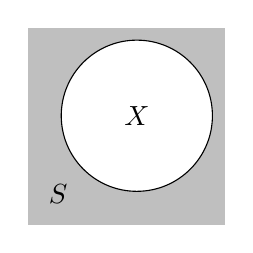
\begin{tikzpicture}[
    	scale=0.8,
    	show background rectangle, 
    	background rectangle/.style={fill=lightgray},
    	box/.style={draw, font=\itshape}
	]
	  \begin{scope}
	    \fill[white] \firstcircle;
      \end{scope}
      \draw \firstcircle node[text=black, fill=white](setx) {$X$};
      \draw node[below of=setx, left of=setx] {$S$};
    \end{tikzpicture}	
}

\card{
	What does $x \in X$ mean?
}{
	$x$ is contained in / is a member of $X$
}

\card{
	What does $x \notin X$ mean?
}{
	$x$ is not a member of $X$
}

\card{
	For each $a$ in $X$, $a \in X \iff a \in Y$.\\
	How is this represented?
}{
	$X=Y$
}

\card{
	How else could we express:\\
	$X \subseteq Y \iff Y \subseteq X$
}{
	$X=Y$
}

\card{
	What does $X \cup Y$ mean?
}{
	The \textbf{union} of the sets $X$ and $Y$.\\
	\vspace{3mm}
    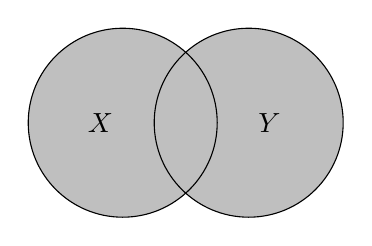
\begin{tikzpicture}
      \begin{scope}
	    \fill[light-gray] \firstcircle;
	    \fill[light-gray] \secondcircle;
      \end{scope}
      \draw \firstcircle node[text=black,right] {$Y$};
      \draw \secondcircle node [text=black,left] {$X$};
    \end{tikzpicture}
}

\card{
	What does $X \cap Y$ mean?
}{
	The \textbf{intersection} of the sets $X$ and $Y$.\\
	\vspace{3mm}
    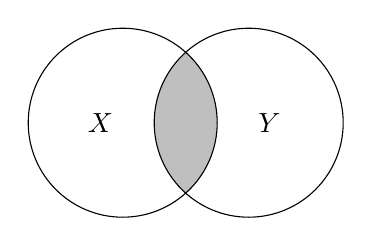
\begin{tikzpicture}
      \begin{scope}
	    \clip \secondcircle;
	    \fill[light-gray] \firstcircle;
      \end{scope}
      \draw \firstcircle node[text=black,right] {$Y$};
      \draw \secondcircle node [text=black,left] {$X$};
    \end{tikzpicture}
}

% Logic functions (truth tables)

\flashcard{
	The truth table for the \texttt{and} function is:
	\begin{tabular}{c|c|c}
		Input 1 & Input 2 & Input 1 \texttt{and} Input 2\\ \hline
		T & T & \blank{T}\\  \hline
		T & F & \blank{F}\\  \hline
		F & T & \blank{F}\\  \hline
		F & F & \blank{F}\\  \hline
	\end{tabular}
}

\flashcard{
	The truth table for the \texttt{or} function is:
	\begin{tabular}{c|c|c}
		Input 1 & Input 2 & Input 1 \texttt{or} Input 2\\ \hline
		T & T & \blank{T}\\  \hline
		T & F & \blank{T}\\  \hline
		F & T & \blank{T}\\  \hline
		F & F & \blank{F}\\  \hline
	\end{tabular}
}

\flashcard{
	The truth table for the \texttt{implies} function is:
	\begin{tabular}{c|c|c}
		Input 1 & Input 2 & Input 1 \texttt{implies} Input 2\\ \hline
		T & T & \blank{T}\\  \hline
		T & F & \blank{F}\\  \hline
		F & T & \blank{T}\\  \hline
		F & F & \blank{T}\\  \hline
	\end{tabular}
}

% Associativity and commutativity

\flashcard{
	An operation is \blank{commutative} if:
	\[
		a1 \circledast a2 = a2 \circledast a1
    \] 
}

\flashcard{
	An operation is \blank{associative} if:
	\[
		(a1 \circledast a2) \circledast a3 = a1 \circledast (a2 \circledast a3)
    \] 
}

% Valid expressions in the formal language

\card{
	Is $(v + w + x)$ a valid expression in the formal language?
}{
	No, there aren't enough brackets.\\
	$((v + w) + x)$ would be valid though!
}

\card{
	Is $(x + 4)$ a valid expression in the formal language?
}{
	No, since $4$ isn't an allowable atom.\\
	$(x + 0)$ would be valid though!
}

\card{
	Is $((x \times 0) + (y + z)))$ a valid expression in the formal language?
}{
	No, since there are too many brackets.\\
	$((x \times 0) + (y + z))$ would be valid though!
}

% Parse trees

\card{
	What expression does this parse tree represent?
	\[
		\infer[(-)]{\parsetreedot} {
			x
			&
			\infer[(\times)]{\parsetreedot} {
				y
				&
				z
			}
		}
	\]
}{
	$(x - (y \times z))$
}

\card{
	Evaluate the following parse tree
	\[
		\infer[(\div)]{\parsetreedot} {
			140
			&
			\infer[(-)]{\parsetreedot} {
				10
				&
				\infer[(\times)]{\parsetreedot} {
					3
					&
					1
				}
			}
		}
	\]
}{
	$(140 \div (10 - (3 \times 1))) = 20$
	\[
		\infer[(\div)]{20} {
			140
			&
			\infer[(-)]{7} {
				10
				&
				\infer[(\times)]{3} {
					3
					&
					1
				}
			}
		}
	\]
}

% Set identities

\card{
	Use the fact that $\cup$ is associative to re-arrange:\\
	$X \cup (Y \cup Z)$ 
}{
	$Y \cup (X \cup Z)$\\
	or\\
	$Z \cup (X \cup Y)$
}

\card{
	Use the fact that $\cap$ is associative to re-arrange:\\
	$X \cap (Y \cap Z)$ 
}{
	$Y \cap (X \cap Z)$\\
	or\\
	$Z \cap (X \cap Y)$
}

\card{
	Use the distributive law on:\\
	$X \cup (Y \cap Z)$ 
}{
	$(X \cap Y) \cup (X \cap Z)$
}

\card{
	Use the distributive law on:\\
	$X \cap (Y \cup Z)$ 
}{
	$(X \cap Y) \cup (X \cap Z)$
}

\card{
	Use absorbsion on:\\
	$X \cup (X \cap Y)$ 
}{
	$X$
}

\card{
	Use absorbsion on:\\
	$X \cap (X \cup Y)$ 
}{
	$X$
}

\card{
	What three things happen when De Morgan's law is applied to an expression?
}{
	\begin{tabularx}{90mm}{l X}
		1. & The expression is negated (involution is applied if it's already negated)\\
		2. &  Each sub expression is negated (again, applying involution)\\
		3. &  Each union inside the expression is turned into an intersection and vice versa\\
	\end{tabularx}
}

\card{
	What does involution mean?
}{
	If an expression is negated twice, they cancel each other out.\\
	$X'' = X$
}

% Logical connectives

\card{
	What is the symbol for logical negation?
}{
	$\neg$	
}

\card{
	What is the symbol for conjunction?
}{
	$\wedge$
}

\card{
	What is the symbol for disjunction?
}{
	$\vee$
}

\card{
	What is the symbol for logical and?
}{
	$\wedge$
}

\card{
	What is the symbol for logical or?
}{
	$\vee$
}

\card{
	What is the symbol for implication?
}{
	$\implies$
}

\card{
	What is the symbol for bi-implication?
}{
	$\iff$
}

\flashcard{
	The truth table for the \texttt{bi-implication} function is:
	\begin{tabular}{c|c|c}
		Input 1 & Input 2 & Input 1 \texttt{$\iff$} Input 2\\ \hline
		T & T & \blank{T}\\  \hline
		T & F & \blank{F}\\  \hline
		F & T & \blank{F}\\  \hline
		F & F & \blank{T}\\  \hline
	\end{tabular}
}

% Tautologies, Satisfiables and Contradictions

\flashcard{An expression is a \blank{tautology} when all of it's possible outcomes are true}

\flashcard{An expression is \blank{satisfiable} when at least one of it's possible outcomes are true}

\flashcard{An expression is a \blank{contradiction} when none of it's possible outcomes are true}

\card{
	What is the notation to say $A$ is a tautology?
}{
	$\models A$
}

\card{
	What is the notation to say $A$ is satisfiable?
}{
	$\not\models \neg A$ 
}

\card{
	What is the notation to say $A$ is a contradiction?
}{
	$\not\models A$
}

% Logical equivalence laws

\card{
	Use the fact that $\vee$ is associative to re-arrange:\\
	$X \vee (Y \vee Z)$ 
}{
	$Y \vee (X \vee Z)$\\
	or\\
	$Z \vee (X \vee Y)$
}

\card{
	Use the fact that $\wedge$ is associative to re-arrange:\\
	$X \wedge (Y \wedge Z)$ 
}{
	$Y \wedge (X \wedge Z)$\\
	or\\
	$Z \wedge (X \wedge Y)$
}

\card{
	What are the two possible rearrangements of $A \implies B$?
}{
	$\neg A \vee B$\\
	$\neg B \implies \neg A$
}

\card{
	What is the rearrangement of $\neg(A \implies B)$
}{
	$A \wedge \neg B$
}

\card{
	What is the rearrangement of $A \implies \neg B?$
}{
	$B \implies \neg A$
}

\card{
	Rearrange $A \iff B$
}{
	$(A \implies B) \wedge (B \implies A)$
}

\card{
	Rearrange $A \iff B$
}{
	$(\neg A \vee B) \wedge (\neg B \vee A)$
}

\card{
	Rearrange $A \iff B$
}{
	$(A \wedge B) \vee (\neg A \wedge \neg B)$
}

\card{
	Rearrange $\neg(A \iff B)$
}{
	$(A \wedge \neg B) \vee (B \wedge \neg A)$
}

\card{
	Rearrange $\neg(A \iff B)$
}{
	$\neg (A \wedge B) \wedge (A \vee B)$
}

% NNF, CNF and DNF

\card{
	What two conditions are there for Negation Normal Form?
}{
	\begin{tabularx}{90mm}{l X}
		1. & The expression is build up of literals using only conjunction and disjunction\\
		2. & Negation can be used, but only on literals, not expressions\\
	\end{tabularx}\\
	\vspace{3mm}
	{\footnotesize N.b. a literal is a formula that is either atomic or the negation of an atomic formula (i.e. $x$ or $\neg x$)}
}

\card{
	What two steps do we do to get an expression into Negation Normal Form?
}{
	\begin{tabularx}{90mm}{l X}
		1. & Remove all implication and bi-implication operations by applying the logical identities\\
		2. & Apply De Morgan's laws to any expressions that are negated\\
	\end{tabularx}
}

\card{
	What three conditions are there for Conjunctive Normal Form?
}{
	\begin{tabularx}{90mm}{l X}
		1. & The formula must be in NNF already\\
		2. & There must be no nested brackets\\
		3. & Conjunction must be used outside of the brackets, and disjunction inside the brackets
	\end{tabularx}
}

\card{
	What two steps do we do to get an expression into Conjunctive Normal Form?
}{
	\begin{tabularx}{90mm}{l X}
		1. & Get rid of nested brackets using identities\\
		2. & Use the distributive identities to bring all the disjunctions inside the conjunctions.
	\end{tabularx}
}

\card{
	What is the CNF test for tautologies?
}{
	Each expression in the formula must have both a literal and the negation of the literal.\\
	\vspace{3mm}
	E.g. $(p_1 \vee p_2 \vee \neg p_1) \wedge (p_3 \vee \neg p_2 \vee p_2)$
}

\card{
	What three conditions are there for Disjunctive Normal Form?
}{
	\begin{tabularx}{90mm}{l X}
		1. & The formula must be in NNF already\\
		2. & There must be no nested brackets\\
		3. & Disjunction must be used outside of the brackets, and conjunction inside the brackets
	\end{tabularx}
}

\card{
	What is the DNF test for contradictions?
}{
	Each expression in the formula must have both a literal and the negation of the literal.\\
	\vspace{3mm}
	E.g. $(p_1 \wedge p_2 \wedge \neg p_1) \vee (p_3 \wedge \neg p_2 \wedge p_2)$
}

% Predicates and quantifiers

\card{
	What is the universal quantifier?
}{
	$\forall$
}

\card{
	What is the existential quantifier?
}{
	$\exists$
}

\card{
	What can we do to a universal quantifier with a negation such as this:\\
	\[
		\neg \forall x P(x)
	\]
}{
	We can turn it into an existential quantifier, such as:\\
	\[
		\exists x \neg 	P(x)
	\]
}

\card{
	What can we do to an existential quantifier with a negation such as this:\\
	\[
		\neg \exists x P(x)
	\]
}{
	We can turn it into a universal quantifier, such as:\\
	\[
		\forall x \neg 	P(x)
	\]
}

% Nasty questions

\card{
	What is the arity of a unary symbol?
}{
	1\\
	\vspace{3mm}
	{\footnotesize Arity - the number of arguments that a function can take}
}

\card{
	Is disjunction inclusive or exclusive?
}{
	Inclusive.
}

\card{
	What does 'iff' mean?
}{
	If and only if.
}

\card{
	What does 'PL' stand for?
}{
	Propositional Logic
}

\card{
	What is a truth valuation?
}{
	A truth valuation is a list of values define the input values for an expression. E.g.:\\
	$(x=T, y=F)$
}

\card{
	If $A \implies B$ is a tautology, what does that mean?
} {
	$A$ and $B$ are logically equivalent.
}

\end{document} 
